\let\negmedspace\undefined
\let\negthickspace\undefined
\documentclass[journal,12pt,twocolumn]{IEEEtran}
%\documentclass[conference]{IEEEtran}
%\IEEEoverridecommandlockouts
% The preceding line is only needed to identify funding in the first footnote. If that is unneeded, please comment it out.
\usepackage{cite}
\usepackage{amsmath,amssymb,amsfonts,amsthm}
\usepackage{caption}
\usepackage{algorithmic}
\usepackage{graphicx}
\usepackage{textcomp}
\usepackage{xcolor}
\usepackage{txfonts}
\usepackage{listings}
\usepackage{enumitem}
\usepackage{mathtools}
\usepackage{gensymb}
\usepackage[breaklinks=true]{hyperref}
\usepackage{tkz-euclide} % loads  TikZ and tkz-base
\usepackage{listings}
\DeclareMathOperator*{\Res}{Res}
%\renewcommand{\baselinestretch}{2}
\renewcommand\thesection{\arabic{section}}
\renewcommand\thesubsection{\thesection.\arabic{subsection}}
\renewcommand\thesubsubsection{\thesubsection.\arabic{subsubsection}}

\renewcommand\thesectiondis{\arabic{section}}
\renewcommand\thesubsectiondis{\thesectiondis.\arabic{subsection}}
\renewcommand\thesubsubsectiondis{\thesubsectiondis.\arabic{subsubsection}}

% correct bad hyphenation here
\hyphenation{op-tical net-works semi-conduc-tor}
\def\inputGnumericTable{}                                 %%

\lstset{
	%language=C,
	frame=single, 
	breaklines=true,
	columns=fullflexible
}
\newcommand{\define}{\stackrel{\triangle}{=}}
\newcommand{\permcomb}[4][0mu]{{{}^{#3}\mkern#1#2_{#4}}}
\newcommand{\comb}[1][-1mu]{\permcomb[#1]{C}}

\begin{document}
	%
	
	
	\newtheorem{theorem}{Theorem}[section]
	\newtheorem{problem}{Problem}
	\newtheorem{proposition}{Proposition}[section]
	\newtheorem{lemma}{Lemma}[section]
	\newtheorem{corollary}[theorem]{Corollary}
	\newtheorem{example}{Example}[section]
	\newtheorem{definition}[problem]{Definition}
	%\newtheorem{thm}{Theorem}[section] 
	%\newtheorem{defn}[thm]{Definition}
	%\newtheorem{algorithm}{Algorithm}[section]
	%\newtheorem{cor}{Corollary}
	\newcommand{\BEQA}{\begin{eqnarray}}
		\newcommand{\EEQA}{\end{eqnarray}}
	%	\newcommand{\define}{\stackrel{\triangle}{=}}
	
	\bibliographystyle{IEEEtran}
	%\bibliographystyle{ieeetr}
	
	
	\providecommand{\mbf}{\mathbf}
	\providecommand{\pr}[1]{\ensuremath{\Pr\left(#1\right)}}
	\providecommand{\qfunc}[1]{\ensuremath{Q\left(#1\right)}}
	\providecommand{\sbrak}[1]{\ensuremath{{}\left[#1\right]}}
	\providecommand{\lsbrak}[1]{\ensuremath{{}\left[#1\right.}}
	\providecommand{\rsbrak}[1]{\ensuremath{{}\left.#1\right]}}
	\providecommand{\brak}[1]{\ensuremath{\left(#1\right)}}
	\providecommand{\lbrak}[1]{\ensuremath{\left(#1\right.}}
	\providecommand{\rbrak}[1]{\ensuremath{\left.#1\right)}}
	\providecommand{\cbrak}[1]{\ensuremath{\left\{#1\right\}}}
	\providecommand{\lcbrak}[1]{\ensuremath{\left\{#1\right.}}
	\providecommand{\rcbrak}[1]{\ensuremath{\left.#1\right\}}}
	\theoremstyle{remark}
	\newtheorem{rem}{Remark}
	\newcommand{\sgn}{\mathop{\mathrm{sgn}}}
	\providecommand{\abs}[1]{\left\vert#1\right\vert}
	\providecommand{\res}[1]{\Res\displaylimits_{#1}} 
	\providecommand{\norm}[1]{\left\lVert#1\right\rVert}
	%\providecommand{\norm}[1]{\lVert#1\rVert}
	\providecommand{\mtx}[1]{\mathbf{#1}}
	\providecommand{\mean}[1]{E\left[ #1 \right]}
	\providecommand{\fourier}{\overset{\mathcal{F}}{ \rightleftharpoons}}
	%\providecommand{\hilbert}{\overset{\mathcal{H}}{ \rightleftharpoons}}
	\providecommand{\system}{\overset{\mathcal{H}}{ \longleftrightarrow}}
	%\newcommand{\solution}[2]{\textbf{Solution:}{#1}}
	\newcommand{\solution}{\noindent \textbf{Solution: }}
	\newcommand{\cosec}{\,\text{cosec}\,}
	\providecommand{\dec}[2]{\ensuremath{\overset{#1}{\underset{#2}{\gtrless}}}}
	\newcommand{\myvec}[1]{\ensuremath{\begin{pmatrix}#1\end{pmatrix}}}
	\newcommand{\mydet}[1]{\ensuremath{\begin{vmatrix}#1\end{vmatrix}}}		
		\vspace{3cm}
		
		\title{
			%	\logo{
				Hardware Assignment - AI1110
				%	}
		}
		\author{K.SaiTeja\\
			AI22BTECH11014
		}	
		
\maketitle

\newpage
\bigskip
\renewcommand{\thefigure}{\theenumi}
\renewcommand{\thetable}{\theenumi}
\textbf{Description:-} \raggedright\\
\textbf{In my assignment I've made a Random number generator using decoder, flip flops, XOR gate, 555IC}
\tableofcontents
\section{Components used}
\begin{table}[htbp]
	\label{tab:Hardware_Assignment}
	%%%%%%%%%%%%%%%%%%%%%%%%%%%%%%%%%%%%%%%%%%%%%%%%%%%%%%%%%%%%%%%%%%%%%%
%%                                                                  %%
%%  This is a LaTeX2e table fragment exported from Gnumeric.        %%
%%                                                                  %%
%%%%%%%%%%%%%%%%%%%%%%%%%%%%%%%%%%%%%%%%%%%%%%%%%%%%%%%%%%%%%%%%%%%%%%
\begin{align}
\begin{tabular}{|l|l|l|}\hline
	Component	&Value &Quantity\\ \hline
	Breadboard & &1 \\ \hline
	Seven Segment Diplay &Common Anode &1 \\ \hline
	Decoder &7447 &1 \\ \hline
	Flip Flop &7474 &2 \\ \hline
	X-OR Gate &7486 &1 \\ \hline
	555 IC & &1 \\ \hline
	Resistor &1 K$\Omega$ &1 \\ \hline
	Capacitor &100 nF &1 \\ \hline
	Capacitor &10 nF &1 \\ \hline
	Jumper Wires & & \\ \hline
\end{tabular}
\end{align}

	\caption{Components used}
\end{table}
\section{Setup}
\begin{enumerate}
\item This circuit uses 5V from microusb.
\item This acts as the Vcc of the circuit.
\item The inner buses on both sides are at Vcc.
\item The lowest bus is GND.
\item The uppermost bus is carrying the Clock signal from the 555 timer.
\end{enumerate}
\section{Procedure}
\begin{enumerate}
	\item I assembled the 555 timer circuit based on the configuration shown in fig 1 
	\begin{figure}[h]
	\begin{center}
		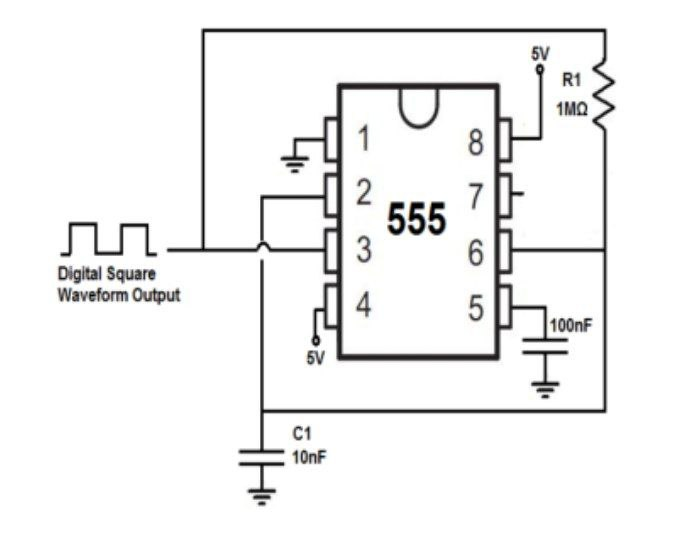
\includegraphics[width=\linewidth]{images/555_timer_circuit.jpg}
		\caption{Connection in 555 timer circuit}
		\label{555_t_c}
		\end{center}
	\end{figure}
	
	\item Next, I linked the Clock output of the 555 timer circuit to the clock signal input of the D-Flip flops.
	
	\item To create the shift registers, I utilized two 7474 ICs, each containing four D-Flip flops, following the circuit arrangement depicted in Figure 3.
	\begin{figure}[h]
	\begin{center}
		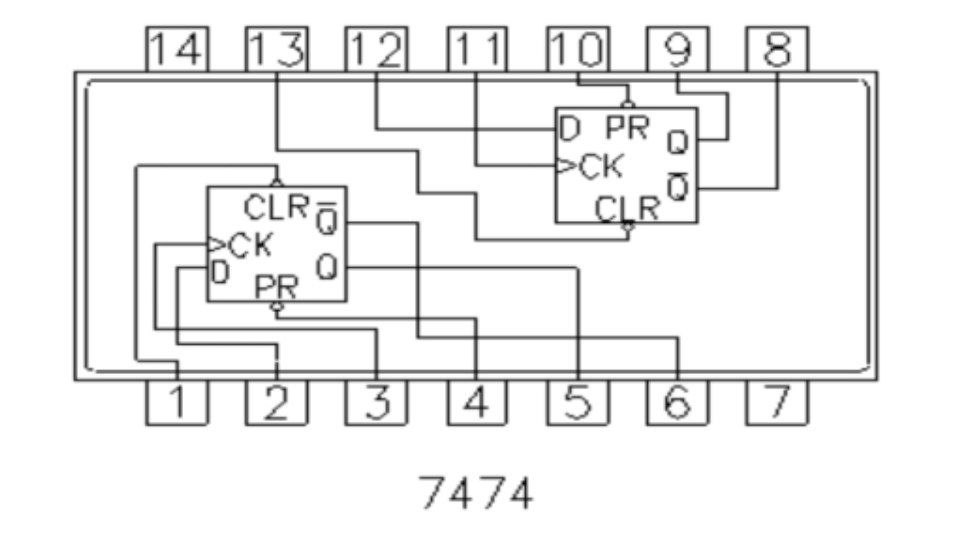
\includegraphics[width=\linewidth]{images/7474.jpg}
		\caption{Connection in 7474 IC}
		\label{7474_IC}
		\end{center}
	\end{figure}

	\item Afterward, I established the connection for the XOR gate using a 7486 IC, as illustrated in Figure 4
	\begin{figure}[h]
	\begin{center}
		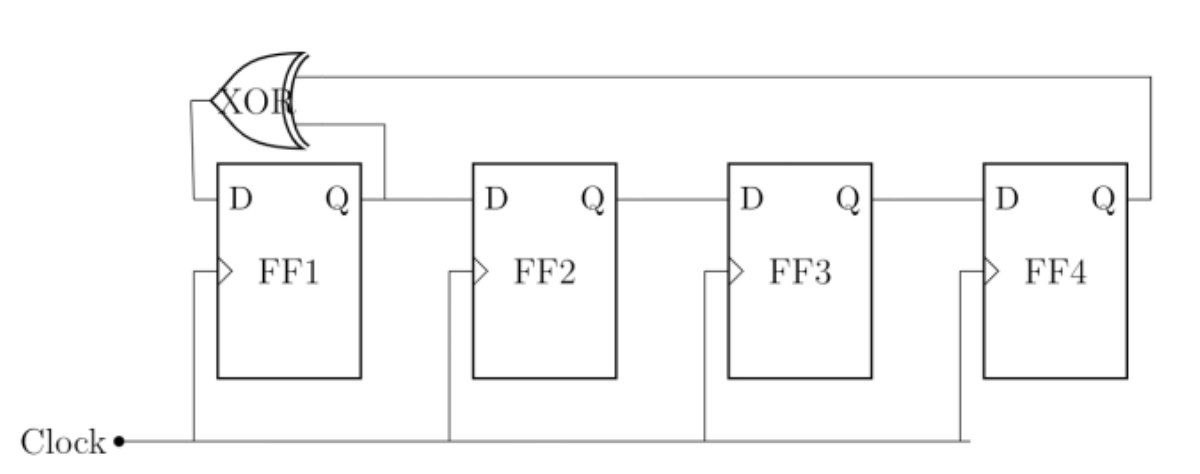
\includegraphics[width=\linewidth]{images/circuit_connections.jpg}
		\caption{Connection in XOR gate}
		\label{XOR}
		\end{center}
	\end{figure}

	\item To connect the decoder (7447 IC), I associated its inputs labeled A, B, C, and D with the outputs $Q_0$, $Q_1$, $Q_2$, and $Q_3$ of the D-Flip flops, respectively, as depicted in Figure 5
	\begin{figure}[h]
	\begin{center}
		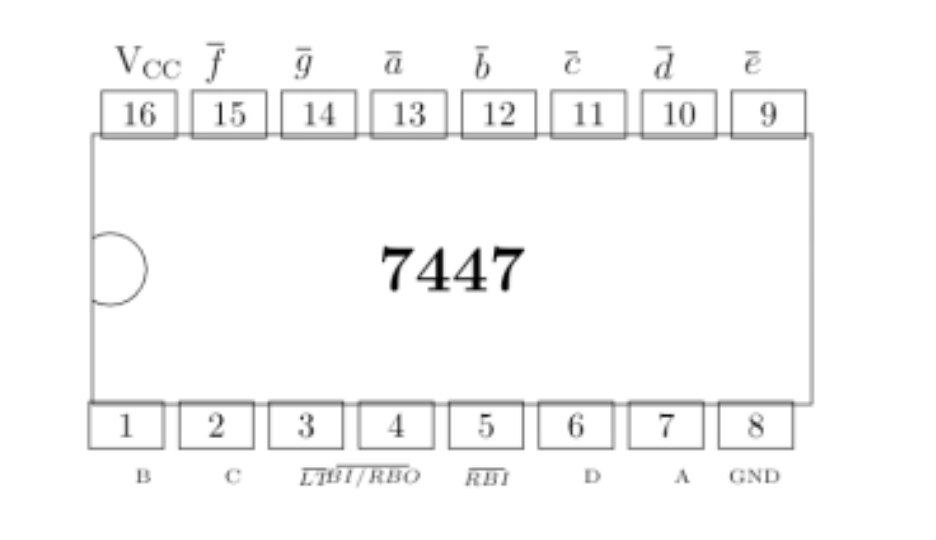
\includegraphics[width=\linewidth]{images/7447.jpg}
		\caption{Connection in Decoder gate}
		\label{7447}
		\end{center}
	\end{figure}
		
	\item According to Figure 6, I connected the decoder (7447 IC) to the seven-segmented display, establishing the appropriate connections. 
	\begin{figure}[h]
	\begin{center}
		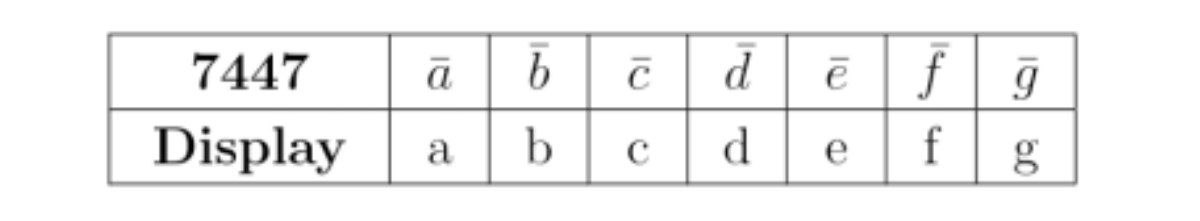
\includegraphics[width=\linewidth]{images/7447_table.jpg}
		\caption{Connection of seven segmented display with decoder}
		\label{table}
		\end{center}
	\end{figure}
	\begin{figure}[h]
	\begin{center}
		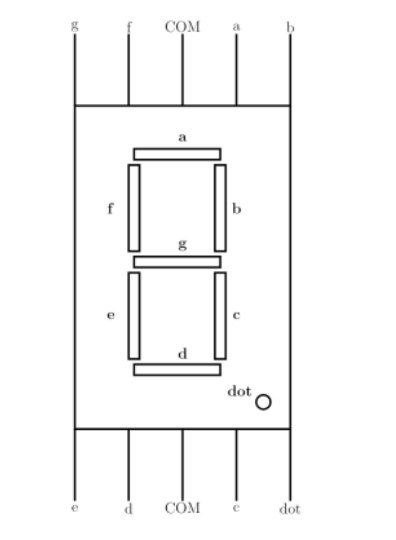
\includegraphics[width=\linewidth]{images/seven_segment_display.jpg}
		\caption{Seven segmented display}
		\label{SSD}
		\end{center}
	\end{figure}

	\item Finally, I interlinked all the individual components and connected the power source to complete the circuit assembly.
\section{Timer}
\begin{enumerate}
\item The time period can be changed using different values of Resistor and Capacitor.
\item As the capacitor advised (10nF and 100nF or 100nF and 100nF) of these the clock speed was too fast and was unable to take the readings, the capacitor
used in their place are 47nF and 470nF.
\item This allows us to get a square pulse of 5V every 0.9 seconds approximately. Which is slow enough to
allow us to take readings from the resistor	
\end{enumerate}	
\section{Output} 
	The circuit generates random numbers on the seven segment display. The output is shown in figure 7
	\begin{figure}[h]
	\begin{center}
		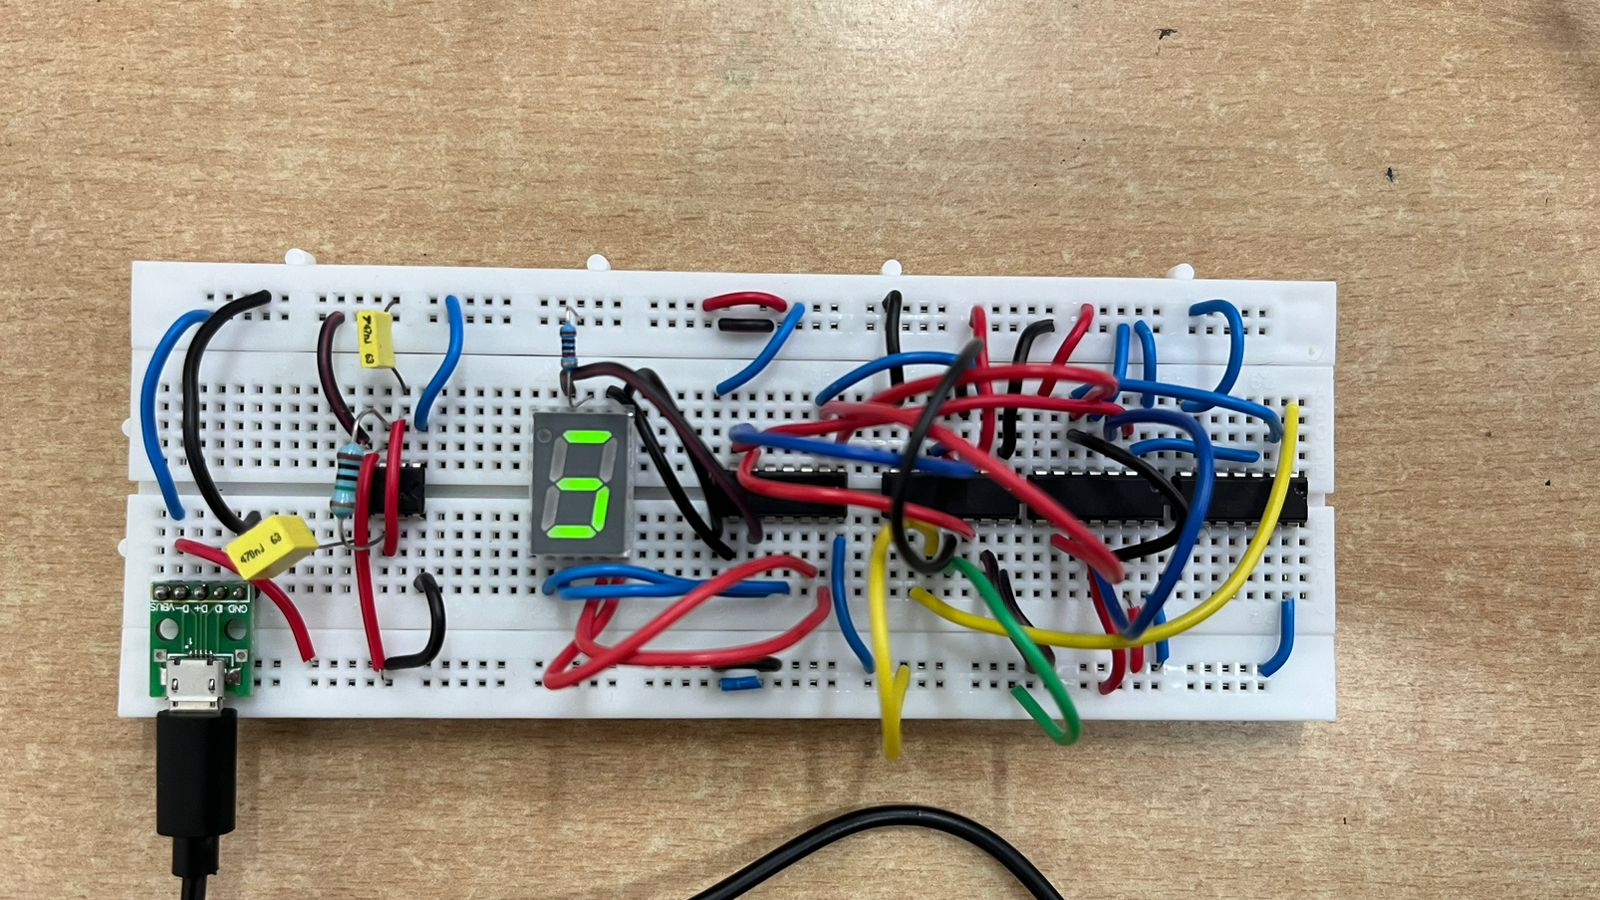
\includegraphics[width = 1\textwidth]{images/fig.jpeg}
		\caption{output}
		\label{final}
		\end{center}
	\end{figure} \\
\section{Block Diagram}
\begin{figure}[h]
\begin{center}
		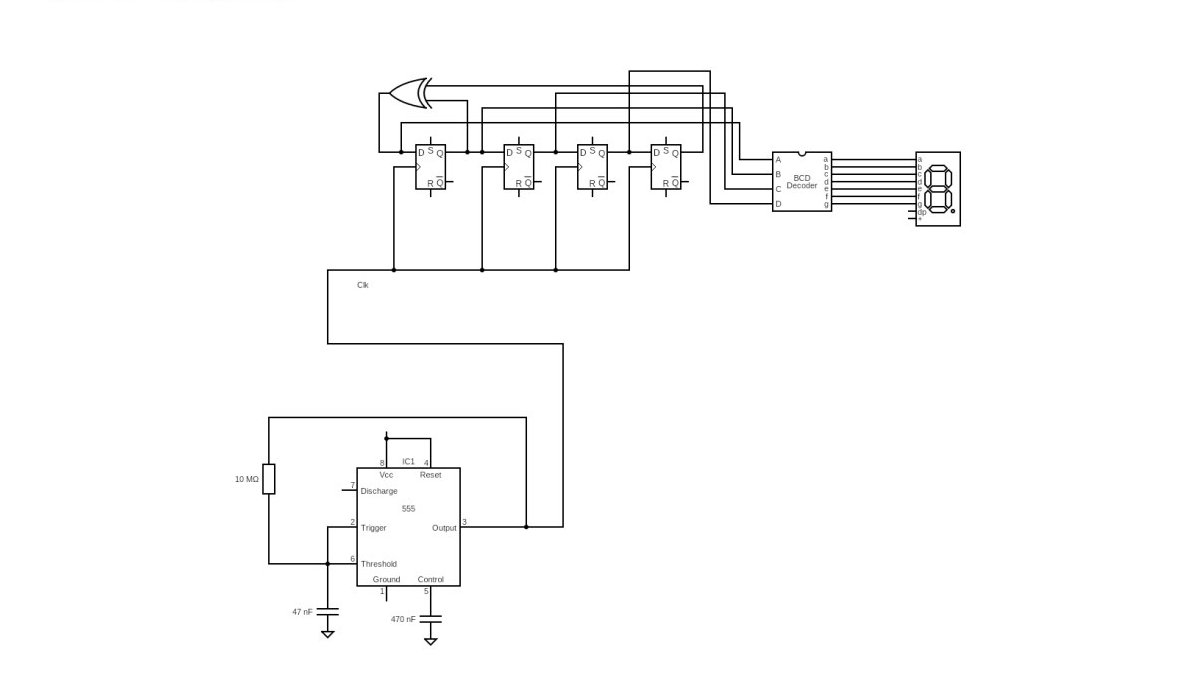
\includegraphics[width= 2\linewidth]{images/fig8.png}
		\caption{Block Diagram}
		\label{Block Diagram}
		\end{center}
	\end{figure}
	
\end{enumerate}
\end{document}